\section{Техническое задание}
\subsection{Основание для разработки}

На основании актуальности проблемы, связанной с частыми нарушениями правил дорожного движения, недостаточным качеством предоставления услуг общественного транспорта и другими аспектами, возникшими в сфере общественного транспорта, было принято решение о разработке веб-приложения для сбора и анализа информации об инцидентах на дорогах общего пользования.

\subsection{Цель и назначение разработки}

Функциональное предназначение разрабатываемого веб-приложения заключается в сборе, анализе и обработке информации, поступающей от пассажиров и граждан, касающейся инцидентов с общественным транспортом. Целью является устранение текущих недочетов, связанных с инцидентами в сфере общественного транспорта.

На текущем этапе разработки приложение будет заниматься обработкой обращений, связанных с инцидентами в городском общественном транспорте безрельсового типа, таких как автобусы, маршрутные такси и троллейбусы. В дальнейшем планируется расширение функционала на все виды общественного транспорта.

Веб-приложение будет обеспечивать эффективную и систематизированную обработку инцидентов, что позволит соответствующим службам и ответственным лицам оперативно реагировать на возникающие проблемы и сокращать их негативное воздействие на пассажиров. В дополнение к этому, приложение будет предоставлять гражданам удобную платформу для обратной связи, способствуя увеличению прозрачности и уровня доверия к деятельности транспортных служб.


Согласно поставленной цели, были сформулированы следующие задачи:
\begin{enumerate}
\item Разработка информационного веб-приложения.
\item Создание базы данных.
\item Внедрение функционала авторизации и регистрации.
\item Реализация функционала для создания и отображения новостной ленты.
\item Осуществление системы загрузки обращений.
\end{enumerate}

В результате выполнения поставленных задач будет создано полноценное информационное веб-приложение, включающее надежную базу данных для хранения, обработки и анализа информации. Пользователи смогут регистрироваться в системе, а также получать доступ к ленте новостей для оперативного информирования о событиях в области транспорта и дорожного движения. Дополнительно, приложение будет оборудовано системой обратной связи, что позволит улучшить взаимодействие между пользователями и транспортными службами.

\subsection{Требования пользователя к интерфейсу}

Веб-приложение должно содержать следующие компоненты:
\begin{itemize}
	\item форма регистрации;
	\item форма авторизации;
	\item форма для добавления обращения;
	\item раздел <<Новостная лента>>, представляющий собой список обращений, успешно прошедших модерацию;
	\item отображение рейтинга водителя;
	\item личный кабинет пользователя;
	\item административная панель.
\end{itemize}

На рисунках 2.1-2.4 представлены макеты интерфейса пользователя программного продукта.
\begin{figure}[H]
	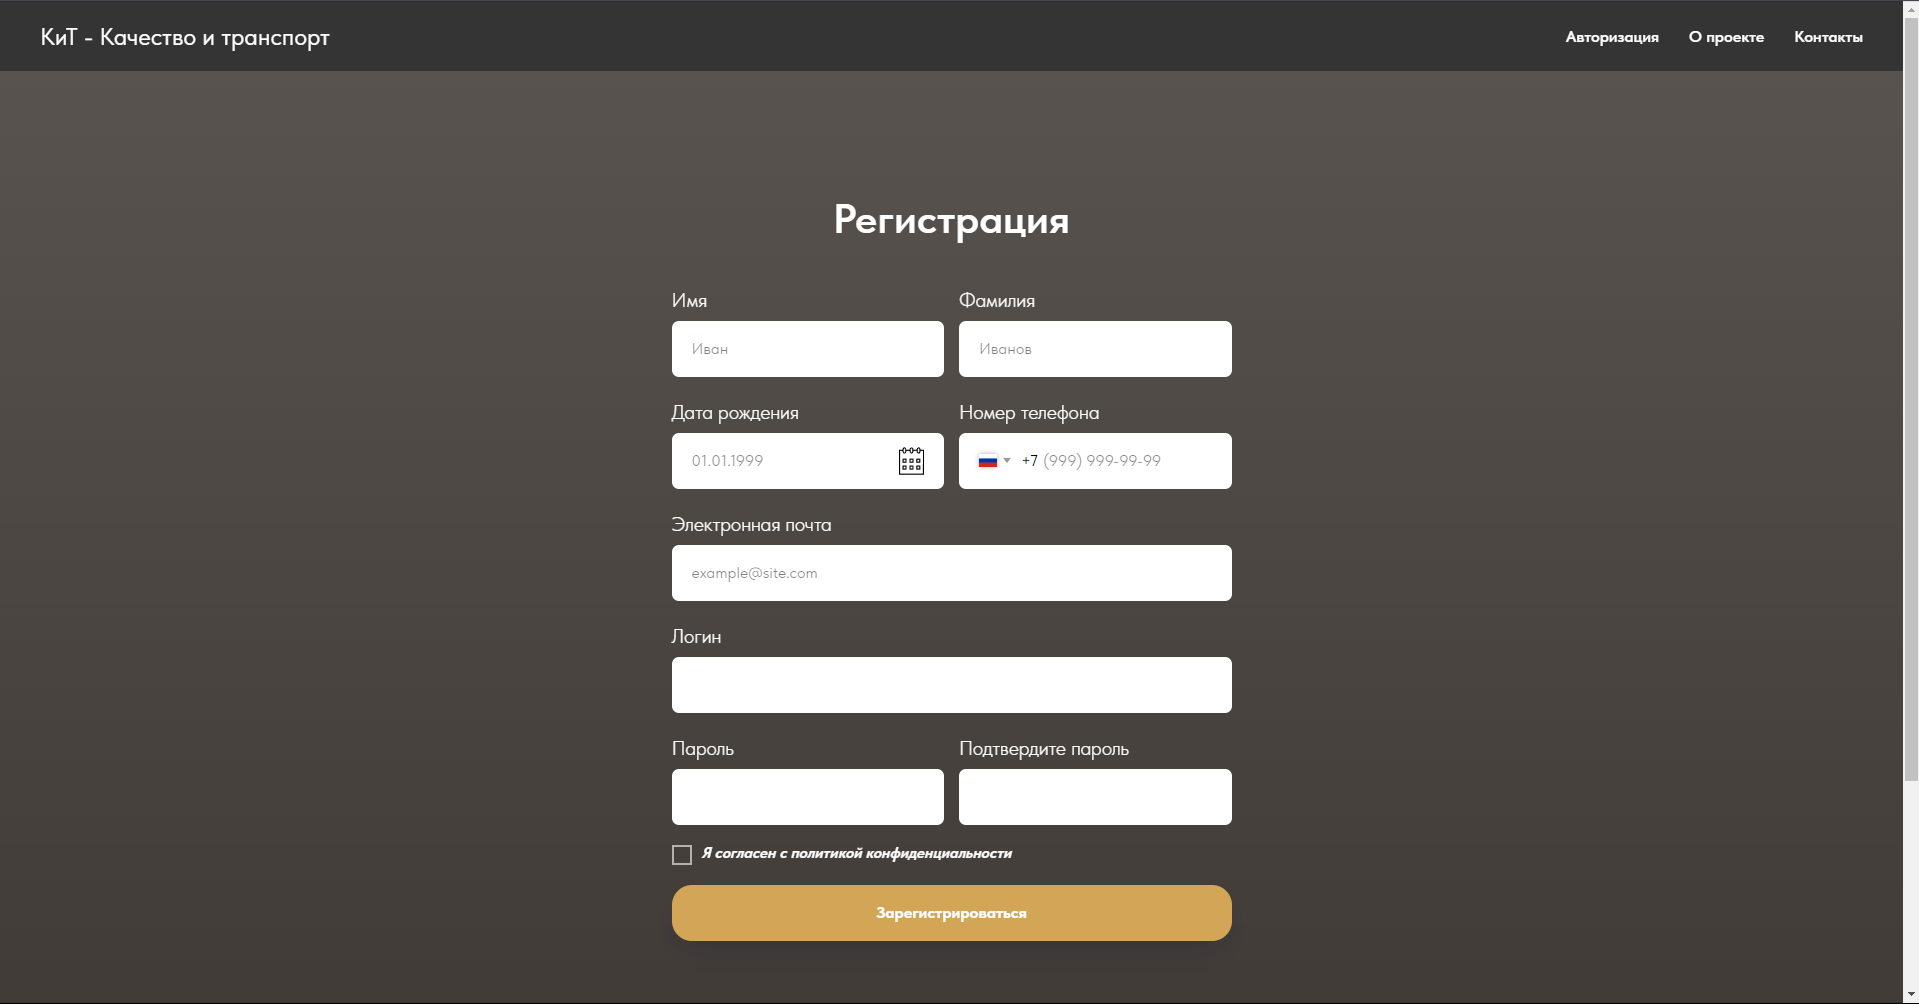
\includegraphics[width=1\linewidth]{Регистрация}
	\caption{Макет формы регистрации}
	\label{templ:image1}
\end{figure}

\begin{figure}[H]
	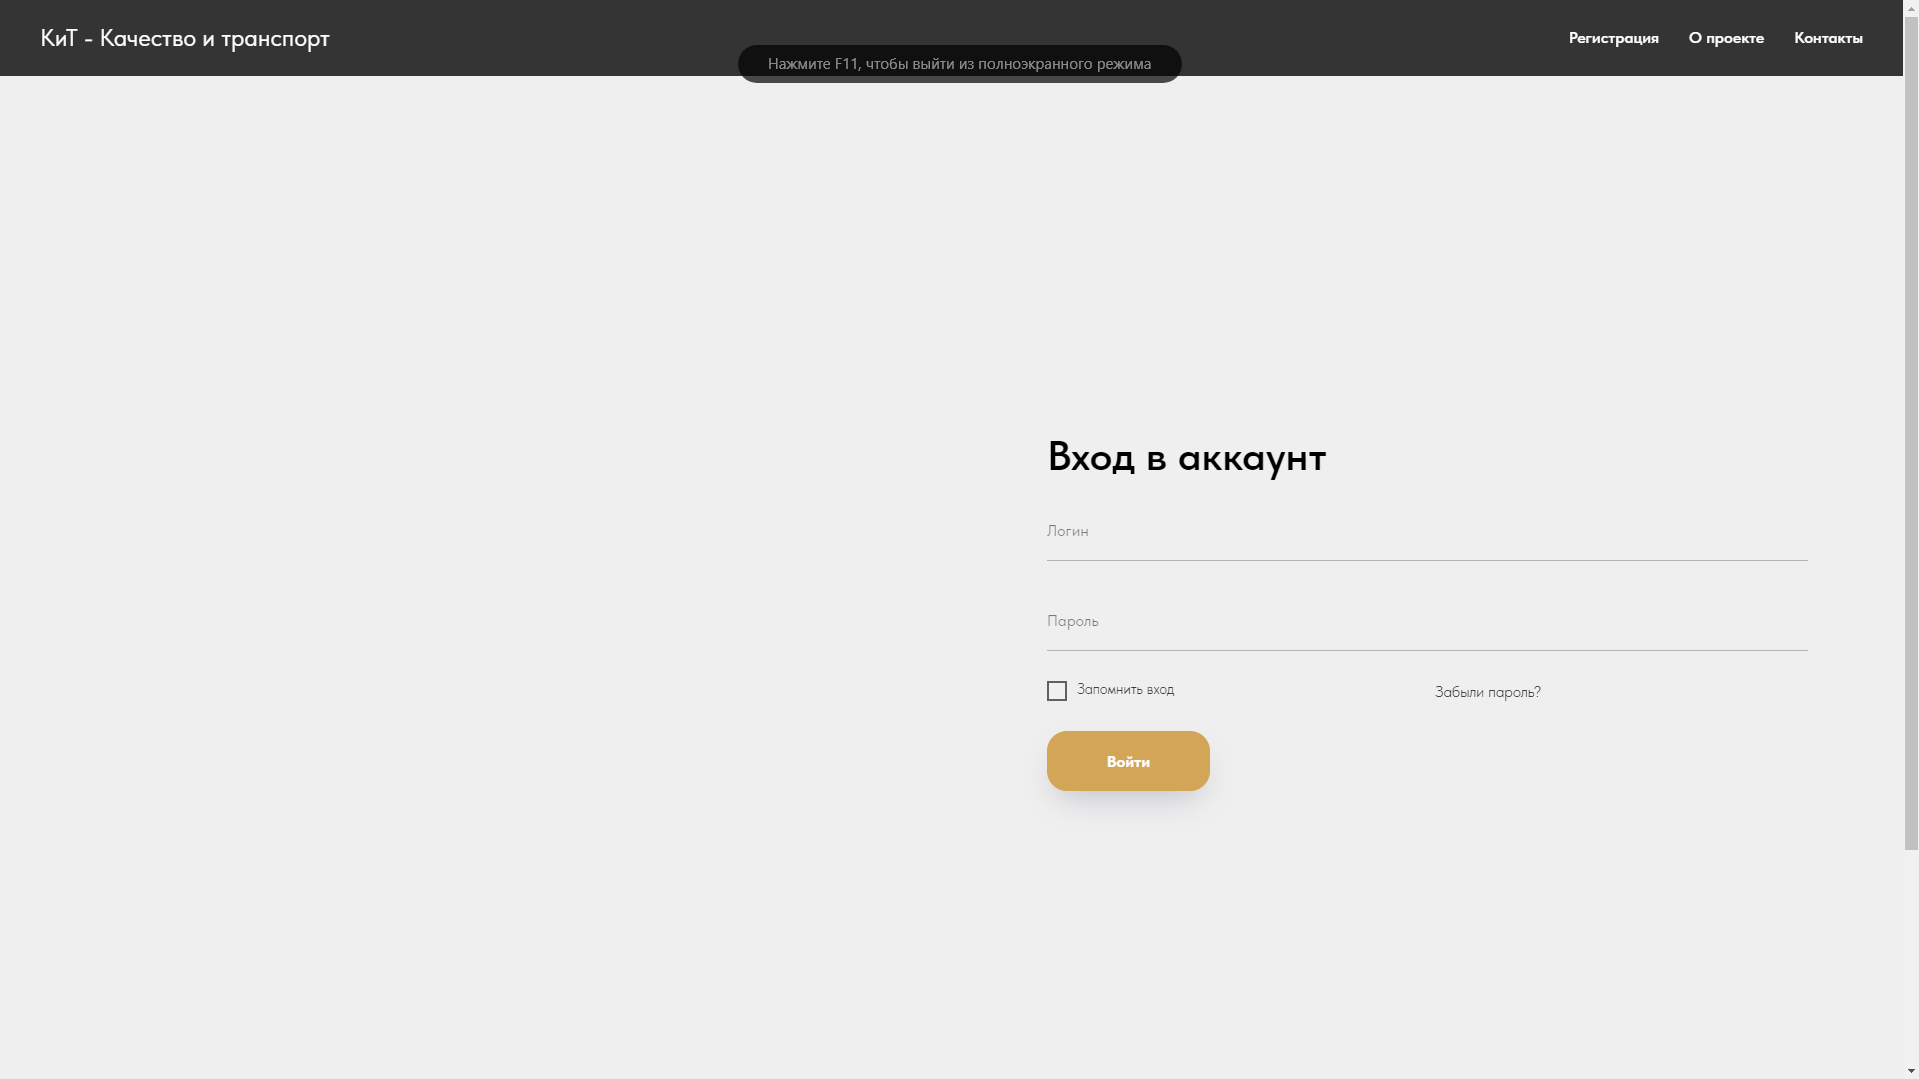
\includegraphics[width=1\linewidth]{Авторизация}
	\caption{Макет формы авторизации}
	\label{templ:image2}
\end{figure}

\begin{figure}[H]
	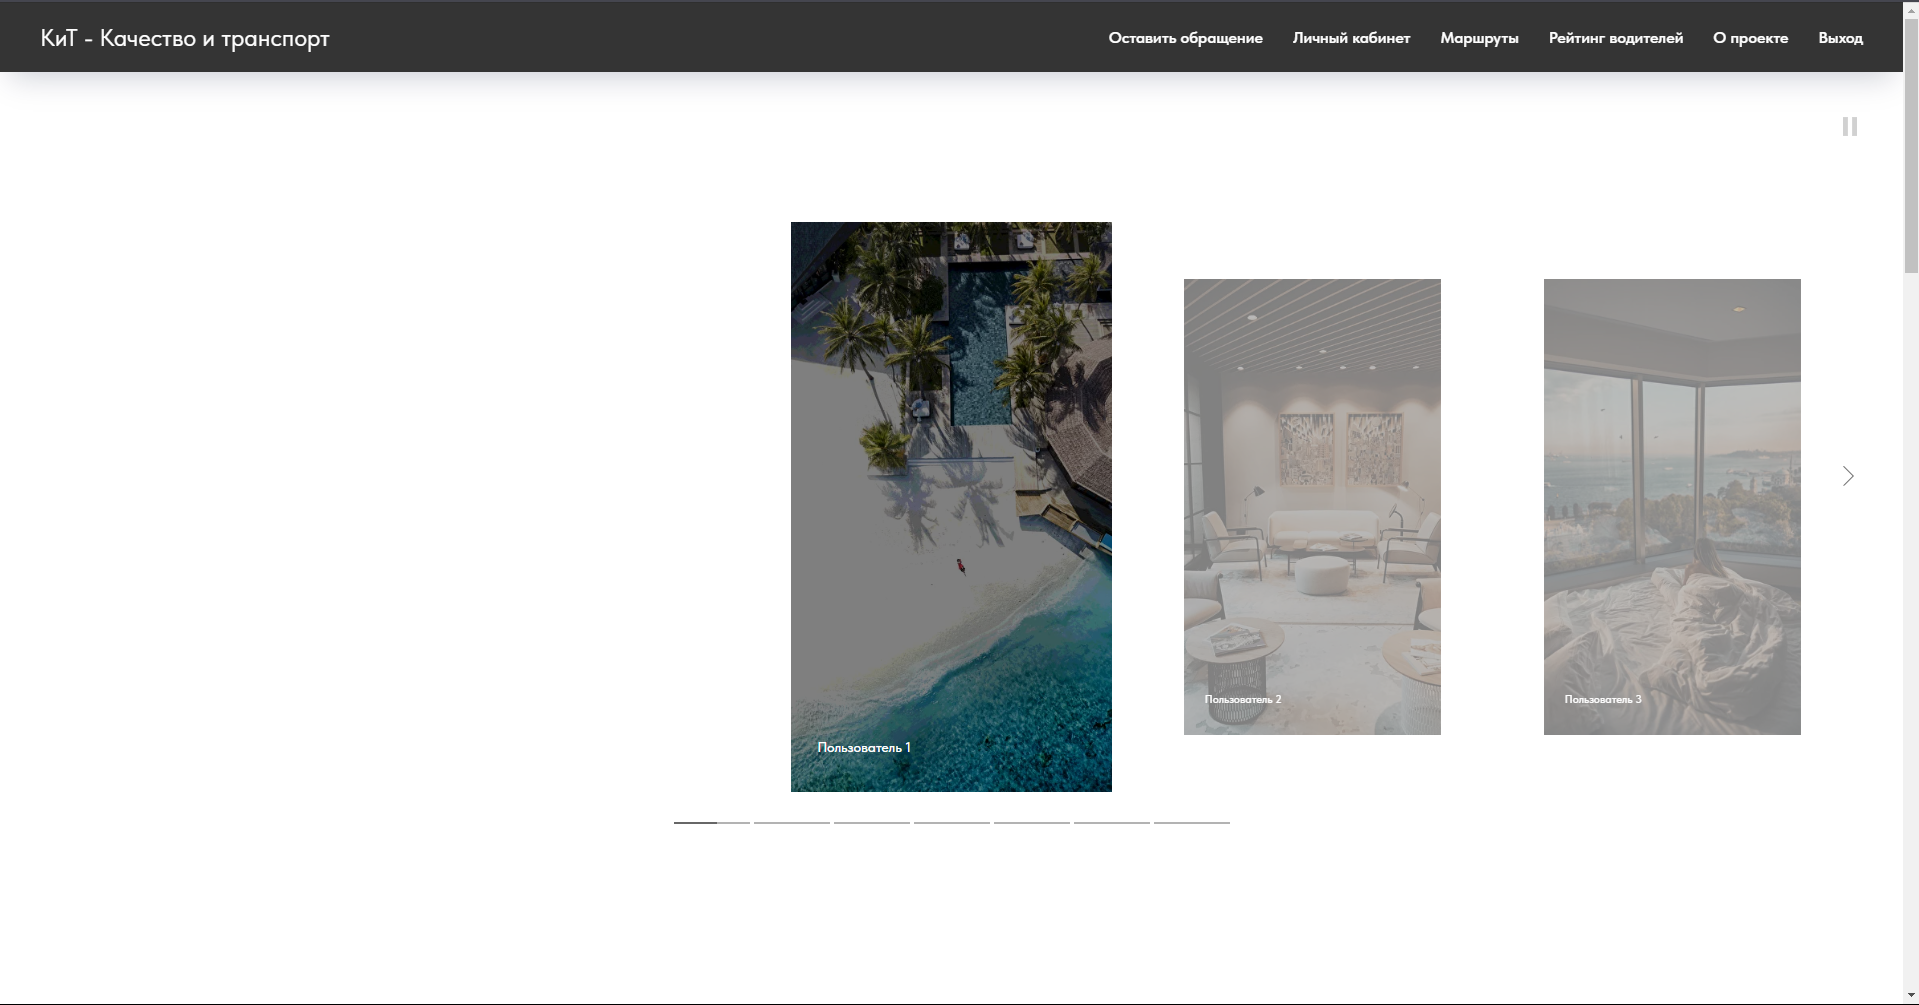
\includegraphics[width=1\linewidth]{Новостная лента}
	\caption{Раздел <<Новостная лента>>}
	\label{templ:image3}
\end{figure}

\begin{figure}[H]
	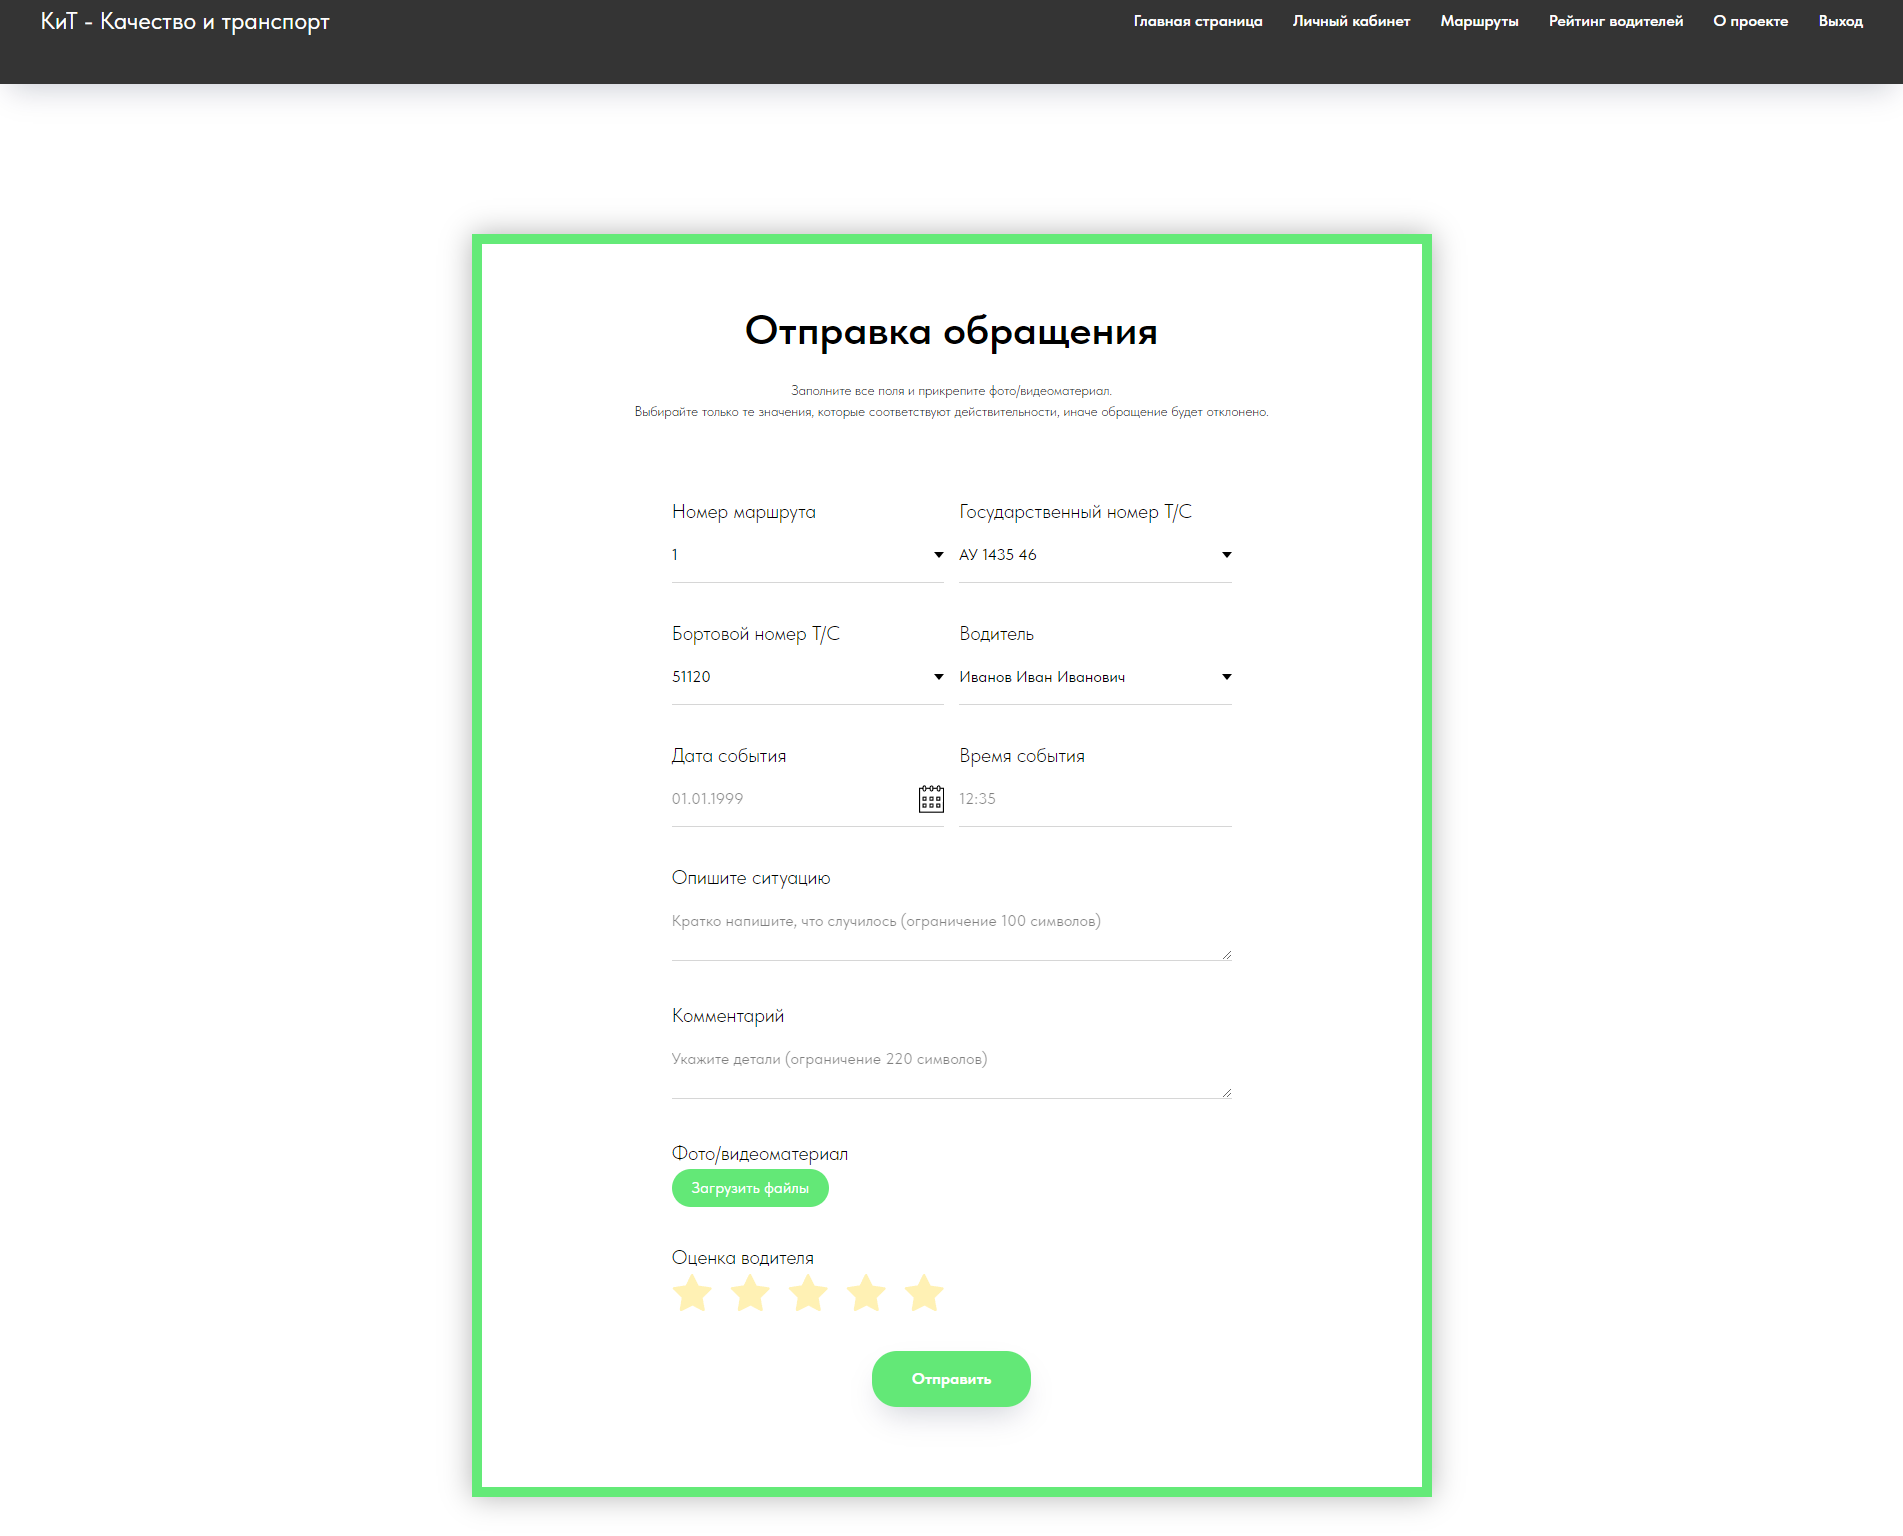
\includegraphics[width=1\linewidth]{Форма обращения}
	\caption{Раздел <<Отправка обращения>>}
	\label{templ:image4}
\end{figure}

\subsection{Моделирование вариантов использования}

Для разрабатываемого веб-приложения была реализована диаграмма прецедентов, которая способствует физической разработке и детальному анализу взаимосвязей объектов. Для построения диаграммы вариантов использования применяется унифицированный язык визуального моделирования UML. 

Диаграмма вариантов использования описывает функциональное назначение разрабатываемой системы, то есть показывает, что система будет делать в процессе своего функционирования. Она представляет собой исходное концептуальное представление системы в процессе проектирования и разработки. В проектируемой системе прецеденты представляют собой действия, предоставляемые системой актерам или сущностям, взаимодействующим с системой. Актером является сущность, взаимодействующая с системой извне, будь то человек или техническое устройство. Прецедент описывает набор действий, которые система выполняет для актера.
На основании анализа предметной области в программе должны быть реализованы следующие прецеденты:
\begin{enumerate}
\item Регистрация аккаунта.
\item Авторизация пользователя.
\item Отправка обращений.
\item Публикация обращений.
\item Просмотр информации в личном кабинете.
\item Модерация обращений.
\end{enumerate}

На рисунке ~\ref{templ:image0} представлены функциональные требования к системе в виде диаграммы прецедентов нотации UML.
\begin{figure}[H]
	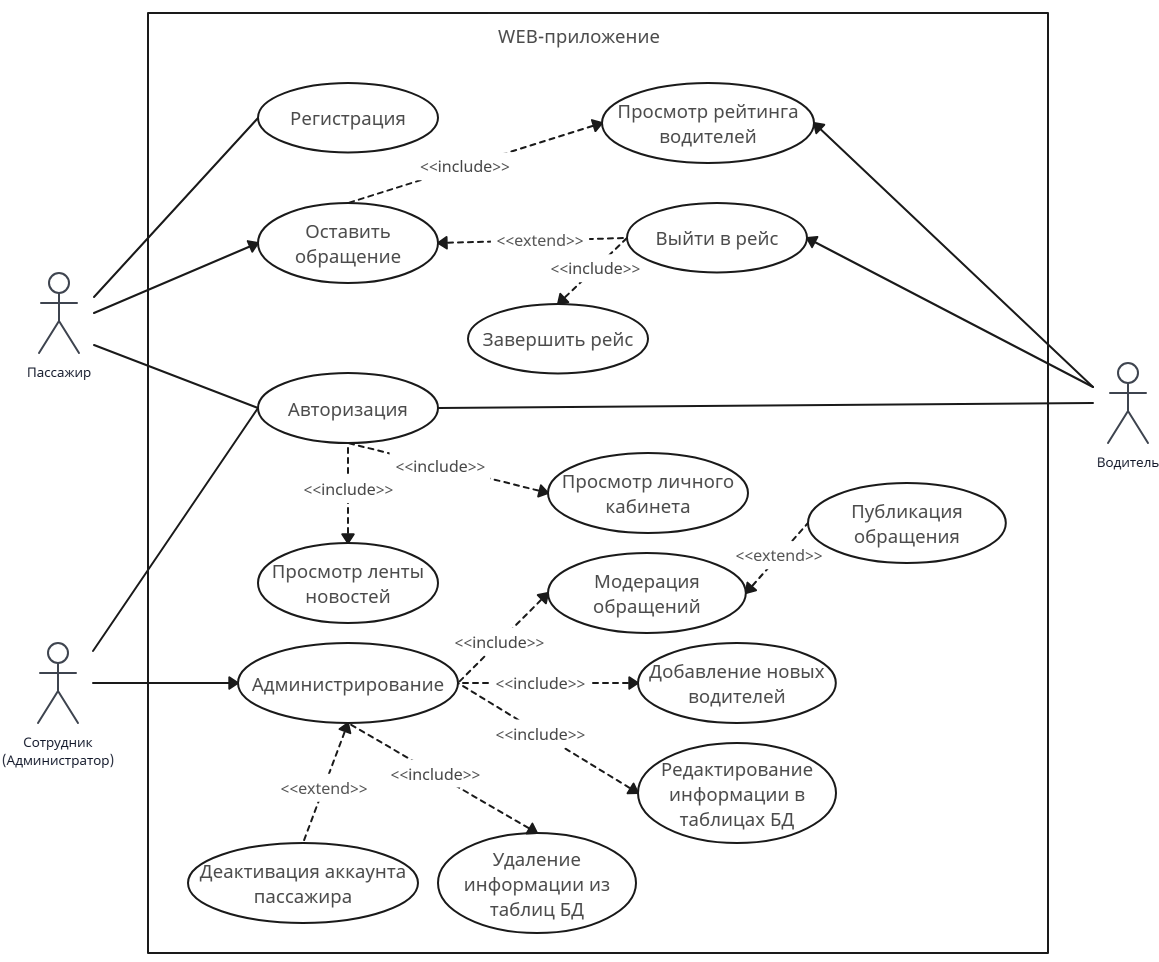
\includegraphics[width=1\linewidth]{Диаграмма прецедентов}
	\caption{Диаграмма прецедентов}
	\label{templ:image0}
\end{figure}

\subsubsection {Вариант использования «Просмотр рейтинга водителей»}
Заинтересованные лица и их требования: Пользователи, желающие ознакомится с рейтингом водителей.

Предусловие: Пользователь заходит в систему под своим аккаунтом.

Постусловие: Пользователь просматривает рейтинг водителей.
Основной успешный сценарий: 

Основной успешный сценарий: 
\begin{enumerate}
	\item Пользователь заходит в раздел «Рейтинг водителей».
	\item Система отображает рейтинговую таблицу водителей, выводя основную информацию: ФИО водителя, номер маршрута, общая оценка. 
\end{enumerate}

\subsubsection {Вариант использования «Добавление новых водителей»}
Заинтересованные лица и их требования: Пользователи, которые несут ответственность за создание аккаунтов новых водителей.

Предусловие: Пользователь вошел в систему под своим аккаунтом, имеющим расширенные права доступа. 

Постусловие: Пользователь создал профиль нового водителя.

Основной успешный сценарий: 
\begin{enumerate}
	\item Пользователь заходит в панель администратора.
	\item Пользователь переходит в раздел «Добавить нового водителя».
	\item Пользователь корректно заполняет все поля формы регистрации. 
	\item Пользователь нажимает на кнопку «Сохранить».
	\item Система создает и открывает аккаунт нового водителя.
\end{enumerate}

\subsubsection {Вариант использования «Регистрация аккаунта»}
Заинтересованные лица и их требования: Пользователи, желающие получить доступ к веб-приложению.

Предусловие: Пользователь открывает страницу регистрации.

Постусловие: Пользователь имеет аккаунт в системе.

Основной успешный сценарий: 
\begin{enumerate}
	\item Пользователь заходит на страницу регистрации.
	\item Пользователь корректно заполняет все поля формы регистрации.
	\item Пользователь нажимает на кнопку «Зарегистрироваться».
	\item Система создает аккаунт пользователя.
\end{enumerate}

\subsubsection {Вариант использования «Авторизация пользователя»}
Заинтересованные лица и их требования: Пользователи, желающие получить доступ к веб-приложению.

Предусловие: Пользователь открывает страницу авторизации.

Постусловие: Пользователь попадает на главную страницу.

Основной успешный сценарий: 
\begin{enumerate}
	\item Пользователь заходит на страницу авторизации.
	\item Пользователь корректно вводит логин и пароль от своего аккаунта в соответствующих полях формы.
	\item Пользователь нажимает на кнопку «Войти».
	\item Система загружает главную страницу.
\end{enumerate}

\subsubsection {Вариант использования «Отправка обращений»}

Заинтересованные лица и их требования: Пользователи, желающие оставить обращение о случившемся инциденте.

Предусловие: Пользователь открывает раздел «Оставить обращение».

Постусловие: Пользователь отправляет обращение в систему.

Основной успешный сценарий: 

\begin{enumerate}
	\item Пользователь заходит в раздел «Оставить обращение».
	\item Пользователь заполняет все необходимые поля.
	\item Пользователь нажимает на кнопку «Отправить».
	\item Система создает новое обращение и отправляет его на проверку администратору.
\end{enumerate}

\subsubsection {Вариант использования «Модерация обращений»}

Заинтересованные лица и их требования: Пользователи, которые несут ответственность за корректность контента обращений.

Предусловие: Пользователь вошел в систему под своим аккаунтом, имеющим расширенные права доступа.

Постусловие: Пользователь допускает обращение для публикации.

Основной успешный сценарий: 

\begin{enumerate}
	\item Пользователь заходит в раздел «Новые обращения».
	\item Пользователь проверяет правильность введённых данных, а также содержание обращения на корректность и достоверность.
	\item Пользователь нажимает на кнопку «Опубликовать». 
	\item Система показывает обращение на главной странице с целью ознакомления для других пользователей.
\end{enumerate}

\subsubsection {Вариант использования «Просмотр информации в личном кабинете»}

Заинтересованные лица и их требования: Пользователи, желающие ознакомится или дополнить информацию о себе в личном кабинете.

Предусловие: Пользователь заходит в систему под своим аккаунтом. 

Постусловие: Пользователь просматривает или дополняет информацию о себе.

Основной успешный сценарий: 

\begin{enumerate}
	\item Пользователь заходит в раздел «Личный кабинет».
	\item Пользователь просматривает имеющуюся информацию и/или добавляет новую информацию.
	\item Пользователь нажимает на кнопку «Сохранить» при добавлении новых данных.
	\item Система выводит сообщение «Данные сохранены», при добавлении новых данных.
\end{enumerate}


\subsection{Требования к оформлению документации}

Разработка программной документации и программного изделия должна производиться согласно ГОСТ 19.102-77 и ГОСТ 34.601-90. Единая система программной документации.
